\documentclass[../Main.tex]{subfiles}

\begin{document}
\chapter{Application Architecture}

\intro{

}

\defn{Software Architecture}{
    The fundamental organization of a system is embodied in its components, their relationships to each other, and to the environment, and the principles guiding its design and evolution.  (ISO/IEC/IEEE 42010, November 2011 )
}

\href{https://arc42.org/overview}{ARC42 Software Architecture Templates}
\href{https://martinfowler.com/eaaCatalog/index.html}{Fowler's Enterprise Architecture}
\href{https://martinfowler.com/eaaDev/uiArchs.html}{Fowler's GUI Architectures}

\section{Architecural Significant Requirements}
\begin{enumerate}
    \item The requirement is directly associated with high business value or business risk
    \item The requirement is a concern of a particularly important stakeholder (for instance, the project sponsor or an external compliance auditor). 
    \item The requirement has runtime Quality-of-Service (QoS) characteristics (e.g., performance needs) that deviate from those already satisfied by the evolving architecture substantially.
    \item  The requirement causes new or deals with one or more existing external dependencies that have unpredictable, unreliable and/or uncontrollable behavior. 
    \item The requirement has a cross-cutting nature and therefore affects multiple parts of the system and their interactions; it may even have system-wide impact. 
    \item The requirement has a first-of-a-kind character: e.g., the team has never built a component before that satisfies this particular requirement. 
    \item The requirement has been troublesome and caused critical situations, budget overruns or client dissatisfaction in a previous project in a similar context. 
\end{enumerate}

\subsection{NFR Catalogs and Taxonomies}
\defn{SMART}{
\begin{description}
    \item[Specific]  Targeting a particular area for improvement
    \item[Measurable] Quantifying, or at least suggesting, an indicator of progress
    \item[Assignable] Defining responsibility clearly
    \item[Realistic] Outlining attainable results with available resources. Time-related: Including a timeline for expected results 
\end{description}
The specific definitions of the words are not fixed.
}

The SMART criteria can be applied to NFR engineering.
\begin{itemize}
    \item Specific: Which feature or part of the system should satisfy the requirement?
    \item Measurable: How can testers and other stakeholders find out whether the requirement is met (or not)? Is the requirement quantified?
    \item A, R, T are requirements engineering and project management concerns: Useful interpretation in our NFR context: Agreed Upon, Realistic, Time-Bound
\end{itemize}

\defn{FURPS+}{
\begin{itemize}
    \item Functionality
    \item Usability
    \item Reliability
    \item Performance
    \item Supportability
\end{itemize}
Plus:
\begin{itemize}
    \item Design constraints
    \item Implementation constraints
    \item Physical constrains
    \item Interface contraints
\end{itemize}
}
\newpage
\subsection{Quality Attribute Scenario (QAS)}
\begin{figure}[H] 
    \centering
    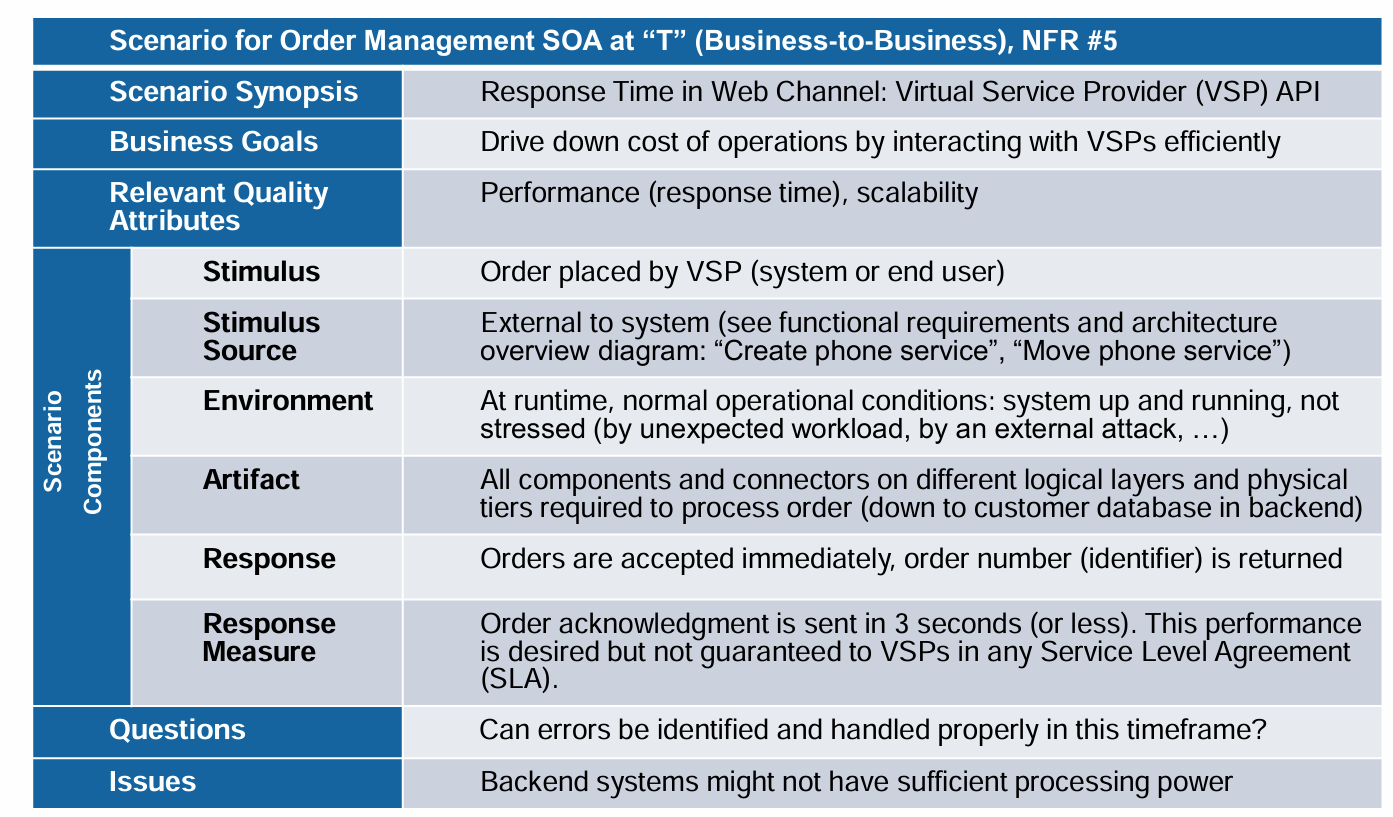
\includegraphics{Images/qas.png}
    \caption{QAS}
    \label{fig:qas}
\end{figure}

Establish three measurable values (M) rather than a single measure that might not be realistic (R) and impossible to agree upon (A) 

\begin{figure}[H]
    \centering
    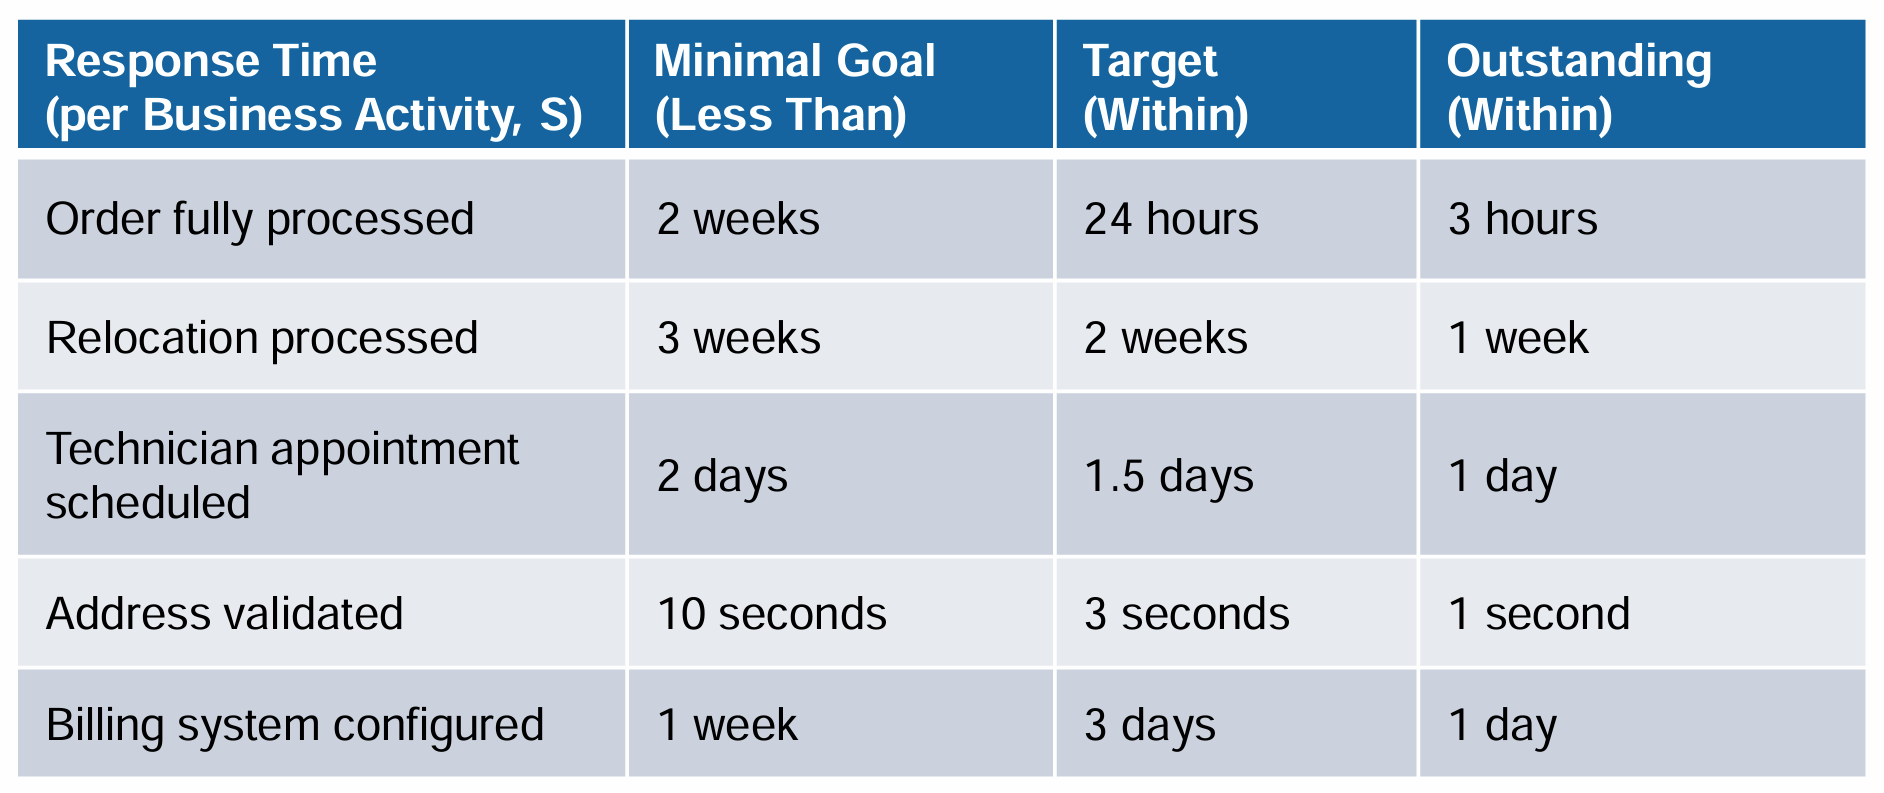
\includegraphics{Images/landingzone.png}
    \caption{Landing Zones}
    \label{fig:landingzones}
\end{figure}

\newpage
\subsection{Twin Peaks}
\begin{figure}[H]
    \centering
    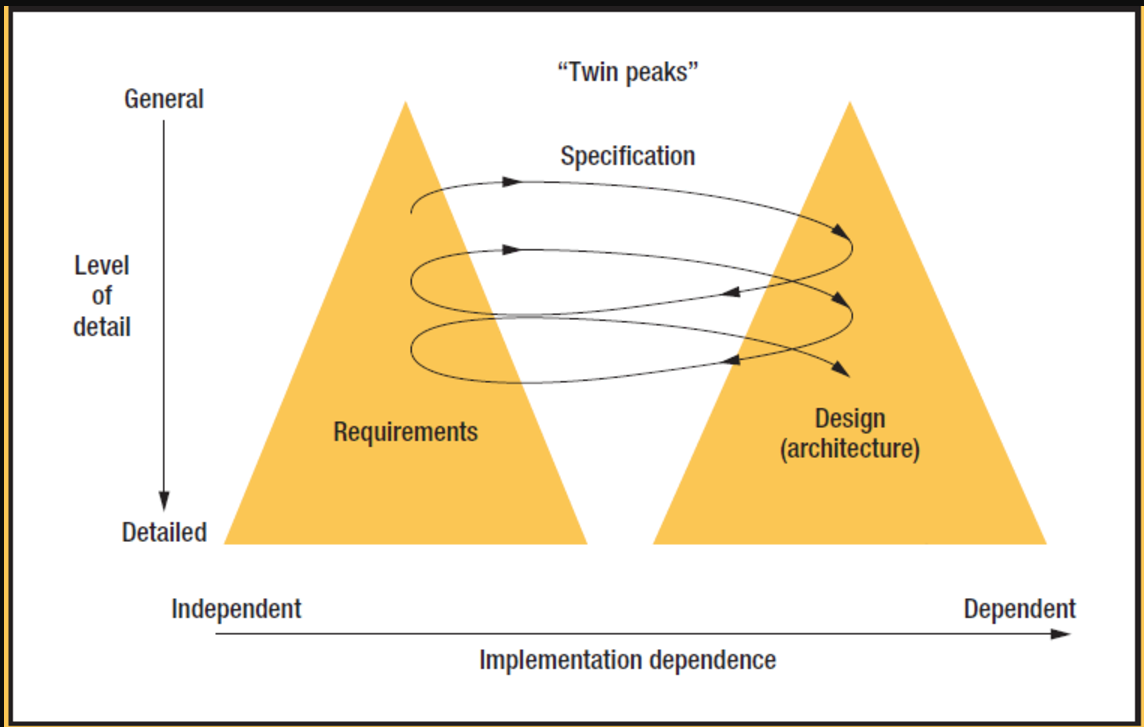
\includegraphics{Images/twinpeak.png}
    \caption{Twin Peak Design}
    \label{fig:twinpeakdesign}
\end{figure}
\newpage

\section{Solution Strategy}
\defn{Solution Strategy}{
fundamental decisions and solution strategies, that shape the system’s architecture. These include:
\begin{itemize}
    \item technology decisions
    \item decisions about the top-level decomposition of the system, e.g. usage of an architectural pattern or design pattern
    \item decisions on how to achieve key quality goals
    \item relevant organizational decisions, e.g. selecting a development process or delegating certain tasks to third parties.
\end{itemize}
 \href{https://docs.arc42.org/section-4/}{ARC42 SS Template}
}

\subsection{Y-Template}
\begin{figure}[H]
    \centering
    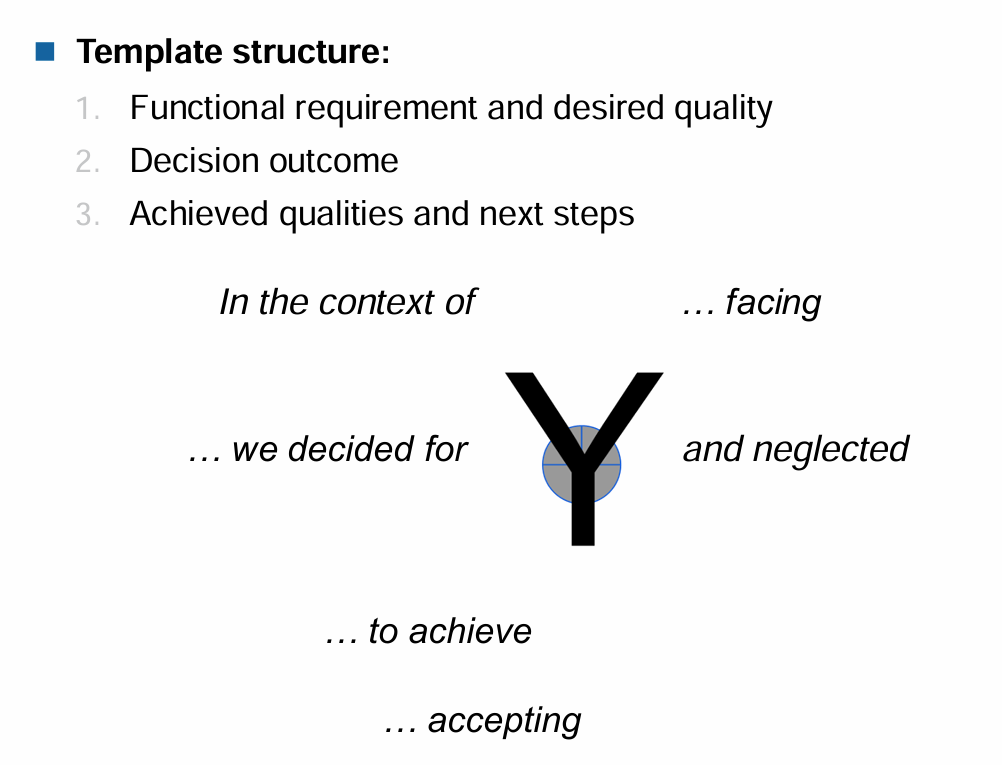
\includegraphics{Images/yarchitecturedesign.png}
    \caption{Y-Template for Architecture Design Decision}
    \label{fig:yarchdesigndecision}
\end{figure}

\newpage
\subsection{Architectural Decision Records}
\href{https://adr.github.io/}{ADR Templates}
\subsection{Logical Layering}
\begin{figure}[H]
    \centering
    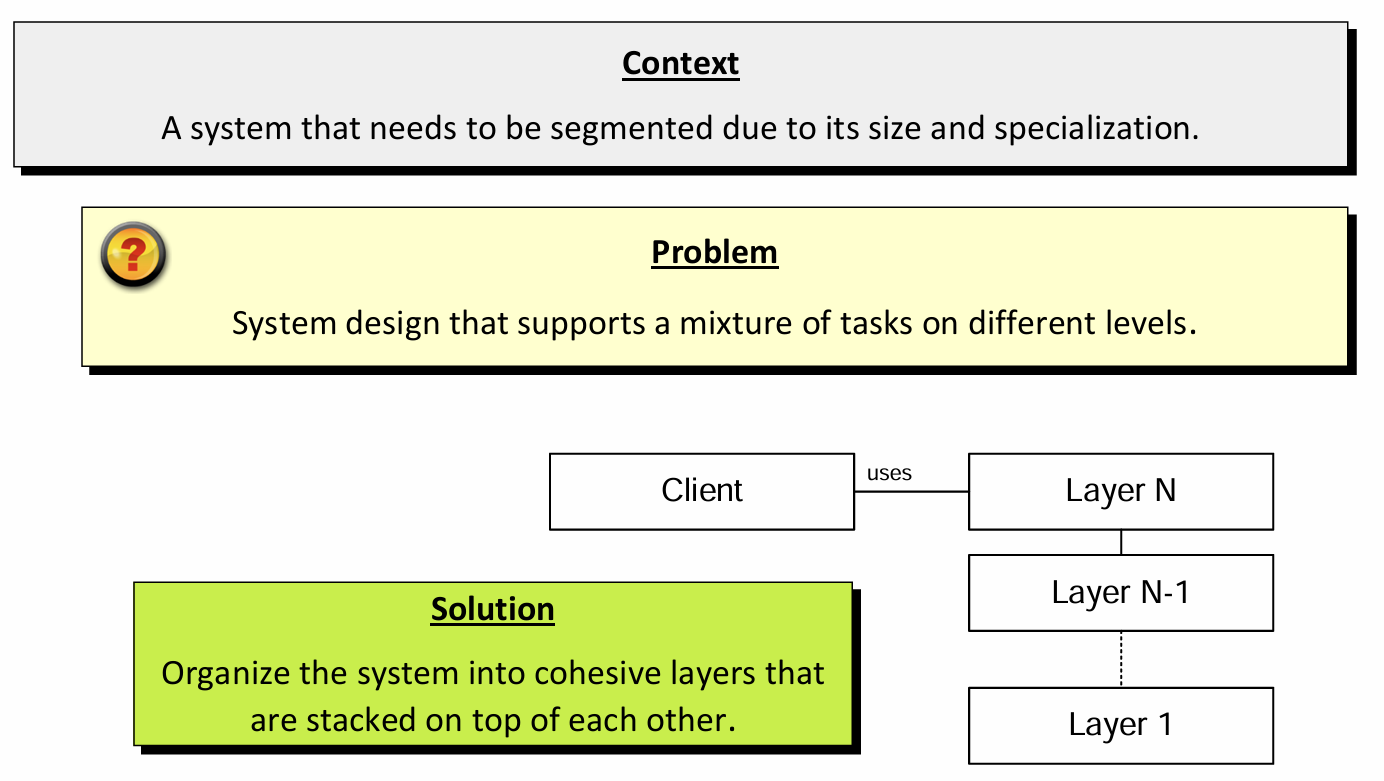
\includegraphics{Images/logicallayering.png}
    \caption{Logical Layering}
    \label{fig:logicallayering}
\end{figure}
\begin{itemize}
    \item Layers separate concerns
    \item Tiers distribute workload
\end{itemize}
\begin{description}
\item[Presentation Layer:] End users and external systems only talk to presentation layer. Rationale: isolation from backend. Presentation layer talks to business logic. Rationale: support multiple presentations of same logic
\item[Business Logic:] Business logic uses data access layer to communicate with database and backend systems. Which can be swapped in and out
\end{description}
The Layers pattern itself does not imply process/server boundary and any use of remoting is optional .
\begin{figure}[H]
    \centering
    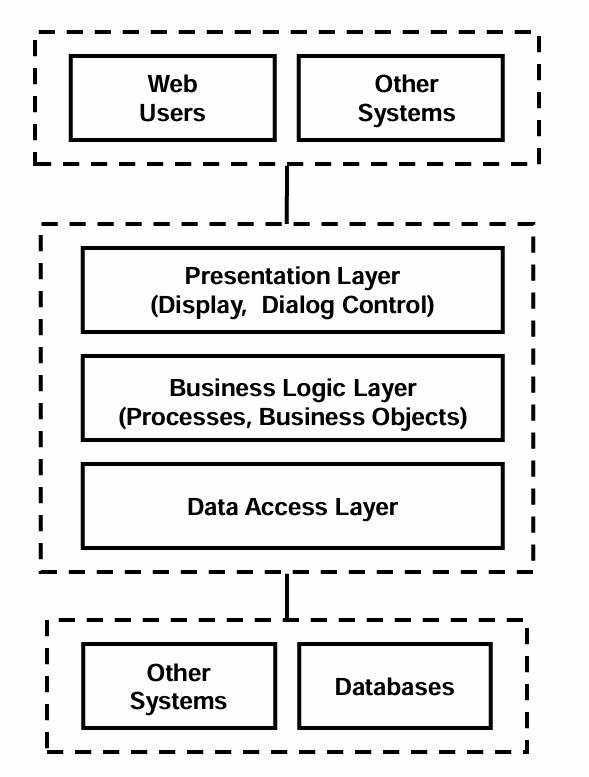
\includegraphics[width=0.5\linewidth]{Images/logicallayer.png}
    \caption{Logical Layers}
    \label{fig:logicallayers}
\end{figure}
Working with three primary logical layers
\begin{itemize}
    \item Presentation
    \item Business logic
    \item Database (access)
\end{itemize}
With many options how to assign layers to tiers: Layer boundary or within layer,  Single or multiple assignments.
\begin{figure}[H]
    \centering
    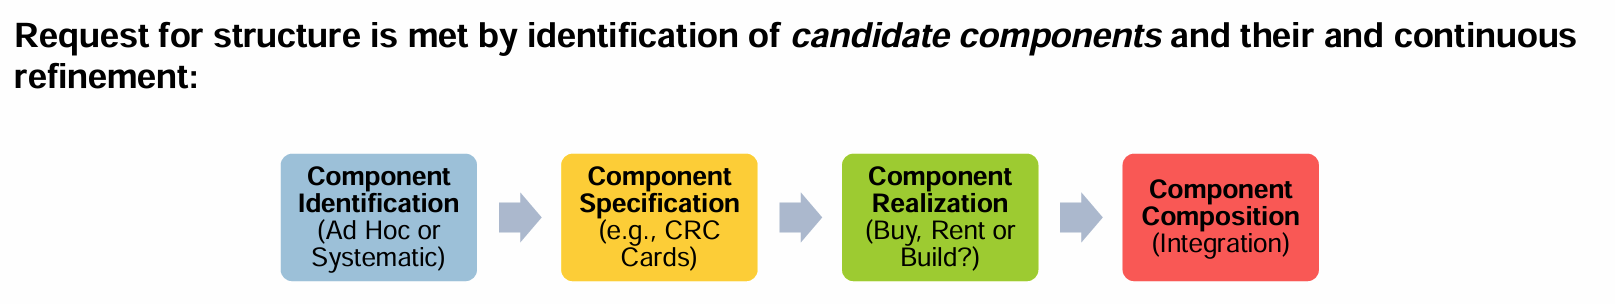
\includegraphics[width=0.5\linewidth]{Images/candidatecomponents.png}
    \caption{Candidate Components}
    \label{fig:ccomponents}
\end{figure}
\newpage
\subsection{Client Server Cuts (CSC)}
\begin{figure}[H]
    \centering
    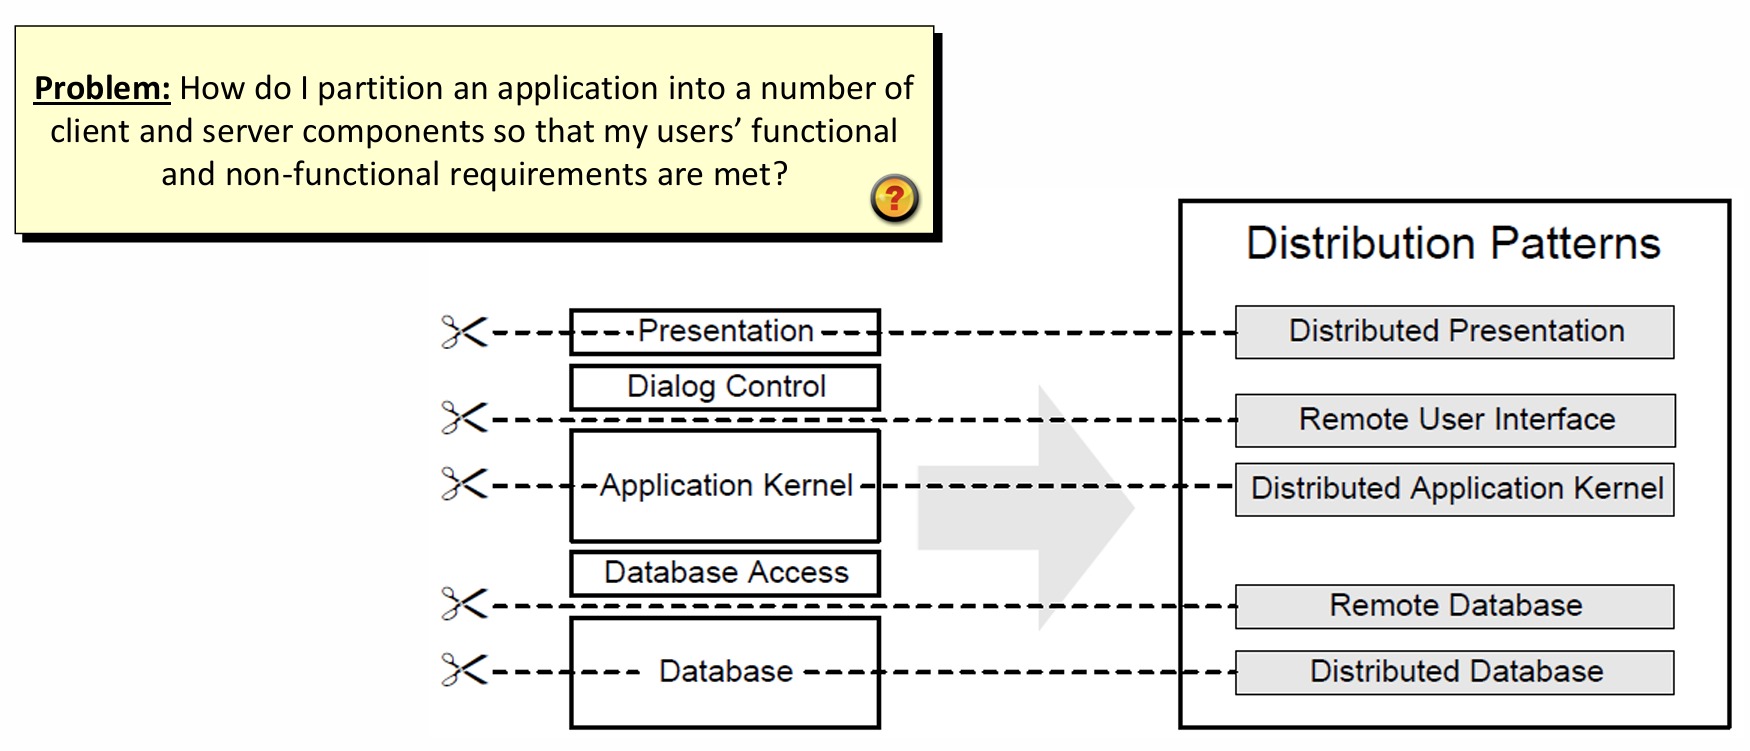
\includegraphics{Images/csc.png}
    \caption{CSC}
    \label{fig:csc}
\end{figure}

\section{Big Architectural Decisions}
\begin{enumerate}
    \item Those with high arch. significance score
    \item  Those requiring financial investment; those with tough consequences
    \item  Those that take a long time to execute upon
    \item Those with many or still unclear outgoing dependencies
    \item Those that take a long time to make according to DoD (ecADR)
    \item Those with a high level of abstraction 
    \item Those with problem/solution space outside of team's comfort zone 
\end{enumerate}
\href{https://github.com/adr/madr}{MADR Templates}
\newpage
\section{Common Components}
\begin{figure}[H]
    \centering
    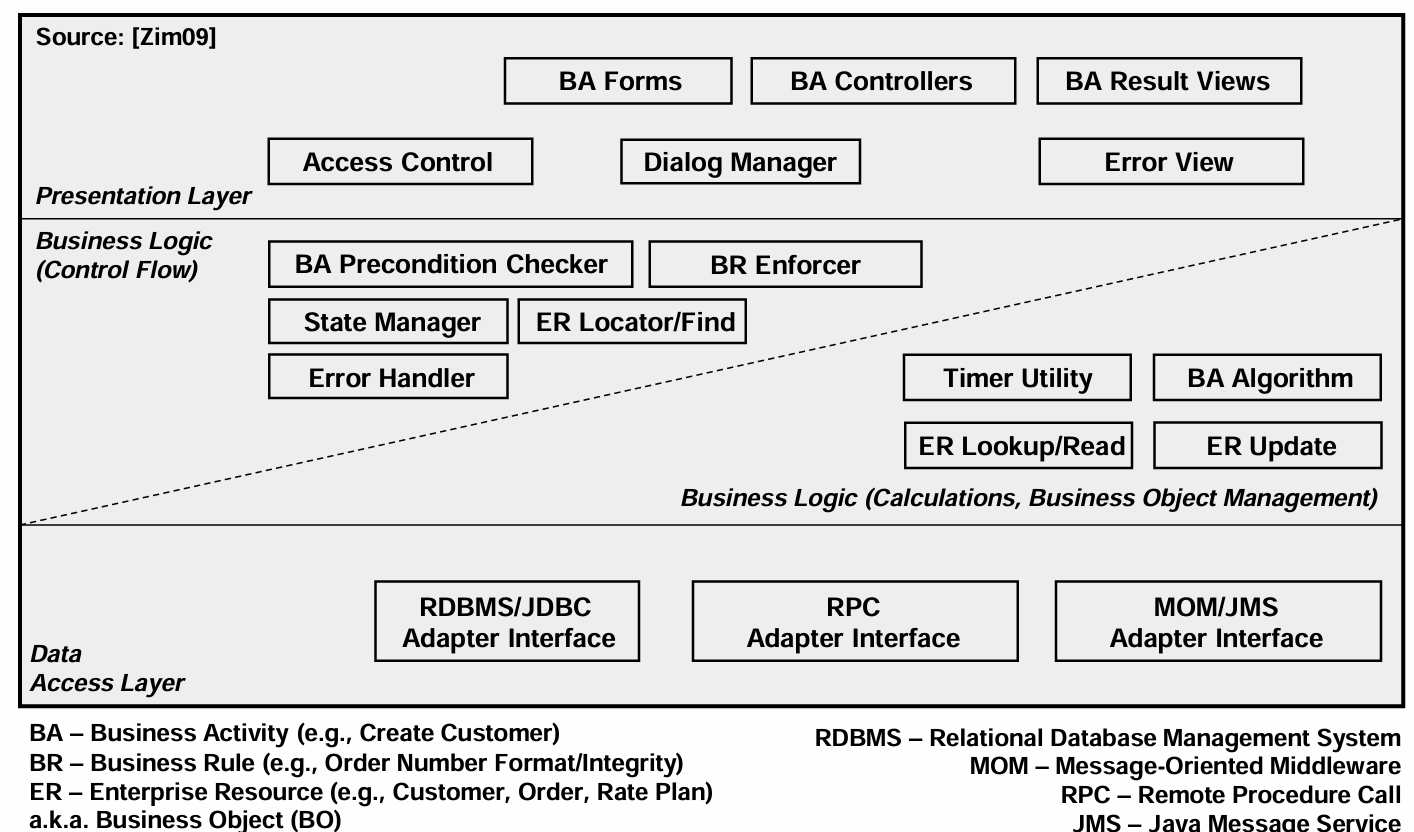
\includegraphics{Images/commoncomponents.png}
    \caption{Common Components}
    \label{fig:commoncomponents}
\end{figure}

\section{Other Tools}
\section{C4 Model}
\defn{C4 Model}{
The C4 model is a software architecture visualization model based on a set of hierarchical abstractions: software systems, containers, components, and code. It uses corresponding hierarchical diagrams—System Context, Container, Component, and Code—to describe these abstractions. The model is intentionally notation-independent and tooling-independent, focusing on clarity and adaptability rather than imposing specific methodologies or tools.
}
C4 model as a "light" alternative to UML. 
\begin{enumerate}
    \item First level of design (solution strategy): containers
    \item Second level of design (refinement): components
    \item Third level of design coded, not diagrammed (construction)
\end{enumerate}

Context matters (the first C in C4), System Context Diagram (SCD) also present in other software engineering and architecture design methods

\begin{figure}[H]
    \centering
    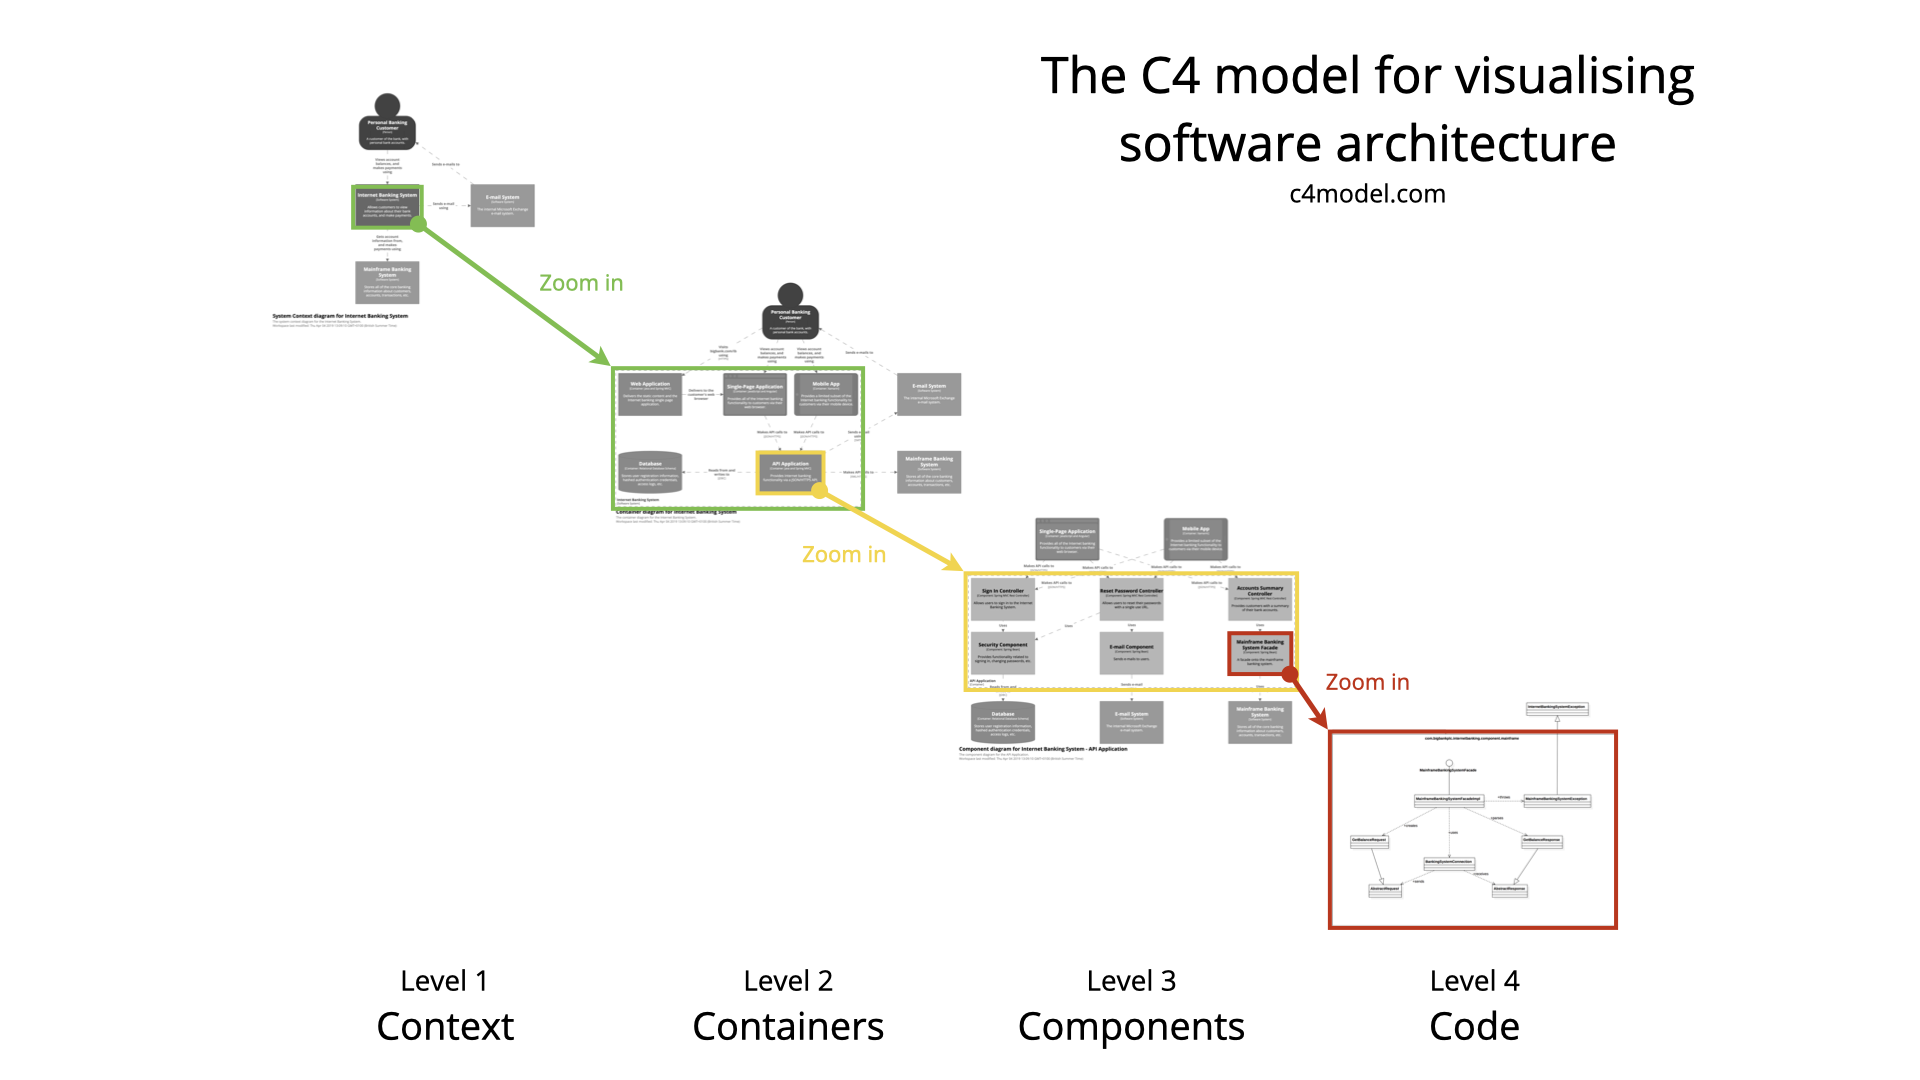
\includegraphics[]{Images/c4-overview.png}
    \caption{C4 Model Overview}
    \label{fig:c4modeloverview}
\end{figure}
\href{https://c4model.com/}{Link to C4 Model Home Page}
\section{Example: Component Interaction Diagram}
\begin{figure}[H]
    \centering
    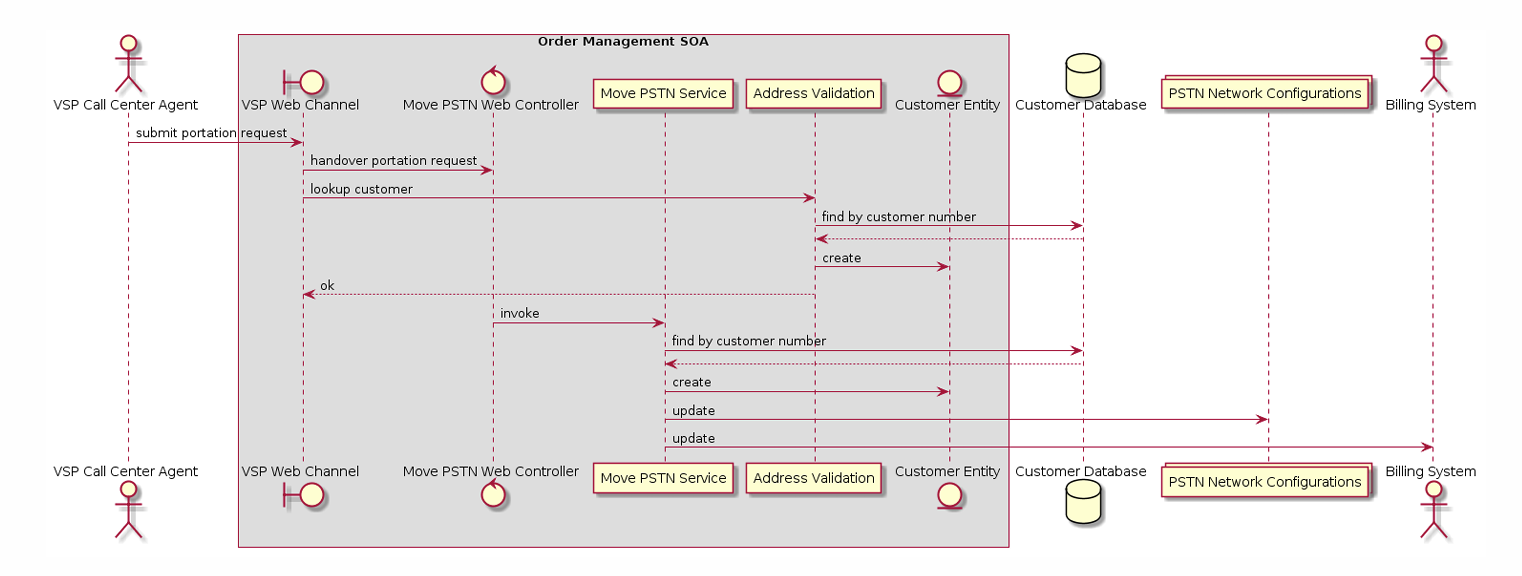
\includegraphics{Images/cid.png}
    \caption{Example Component Interaction Diagram}
    \label{fig:examplecid}
\end{figure}
\newpage
\section{Onion}
\begin{figure}[H]
    \centering
    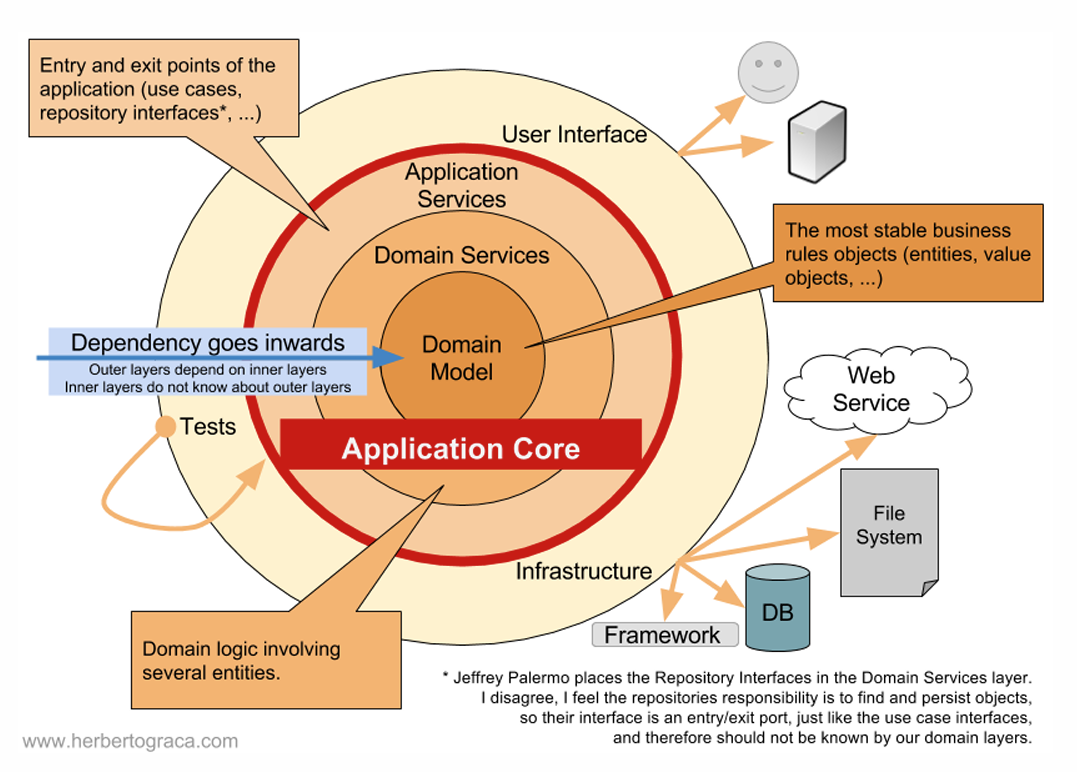
\includegraphics{Images/onion.png}
    \caption{Onion Architecture}
    \label{fig:onionarch}
\end{figure}
\newpage
\section{Story Splitting Flowchart}
\begin{figure}[H]
    \centering
    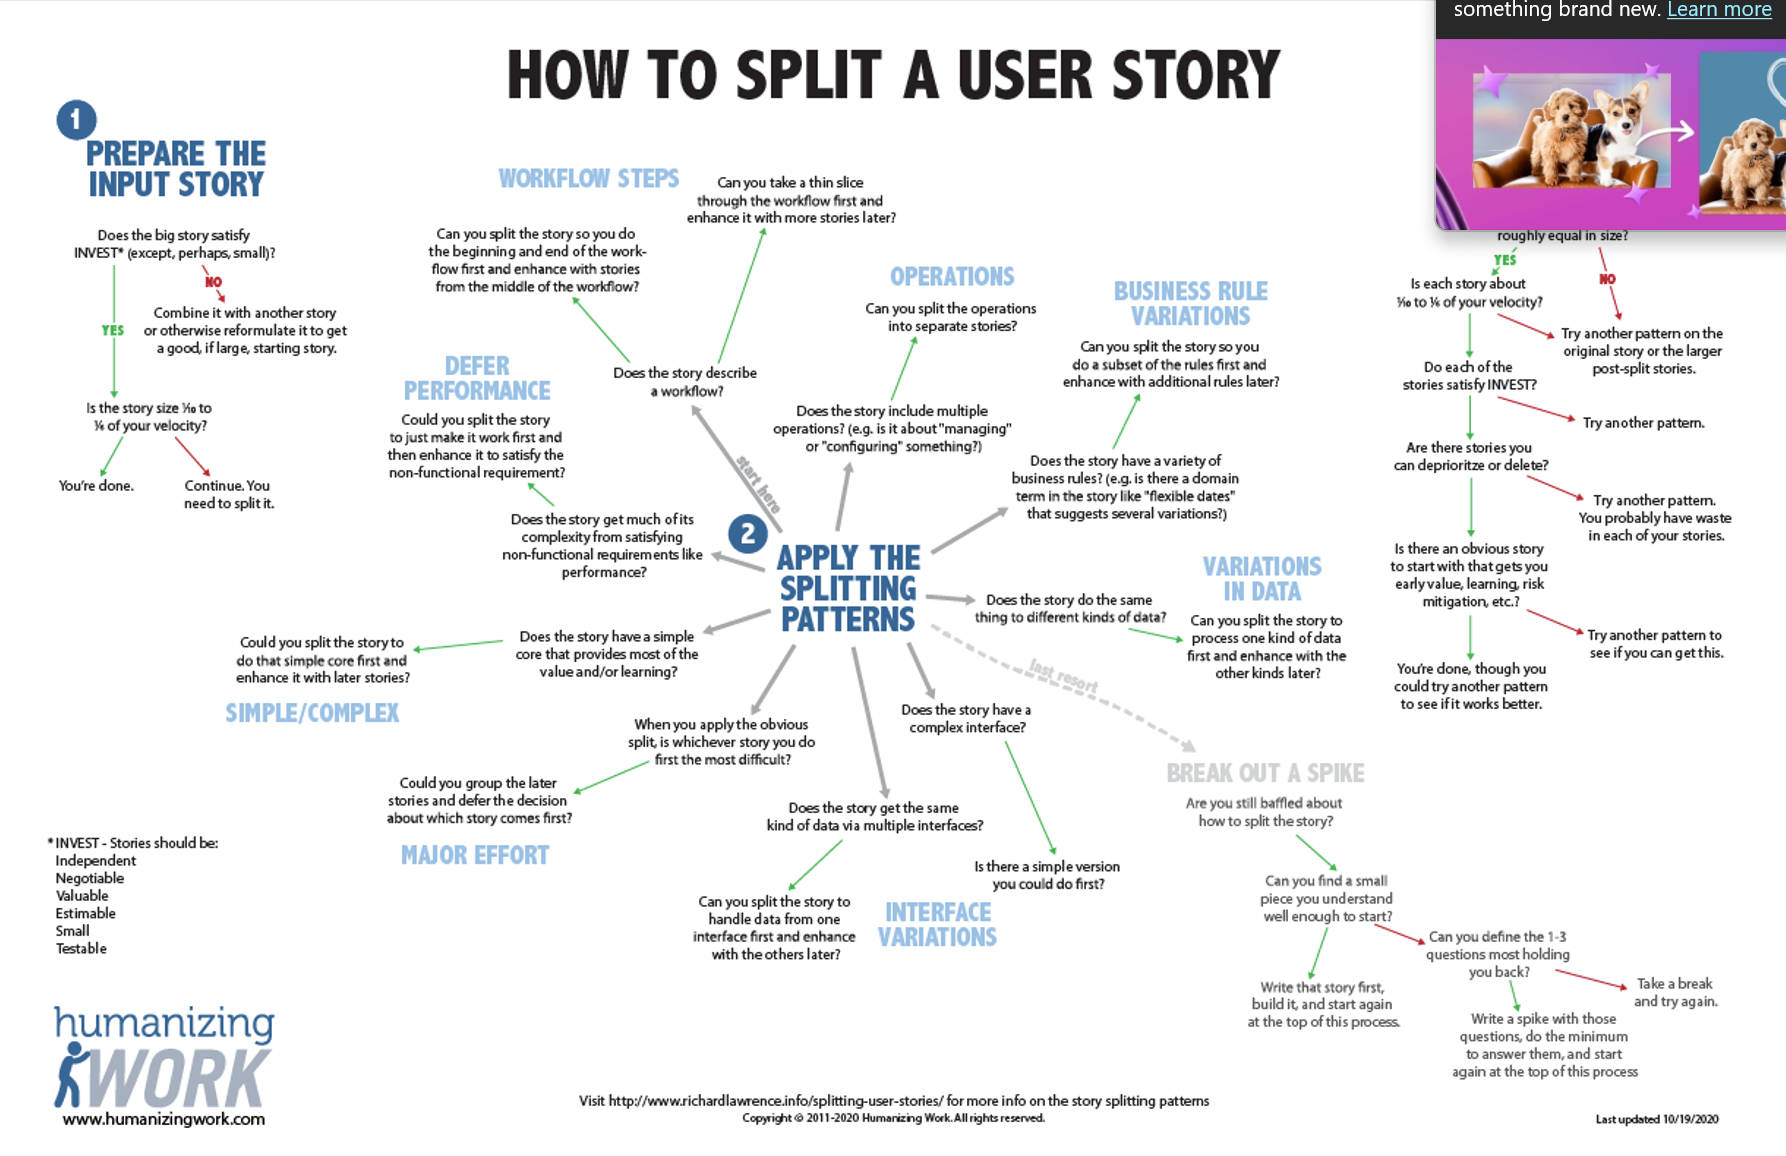
\includegraphics[angle=90,height=1\textwidth]{Images/storysplitting.png}
    \caption{Story Splitting Flowchart}
    \label{fig:storysplit}
\end{figure}
\newpage
\begin{figure}[H]
    \centering
    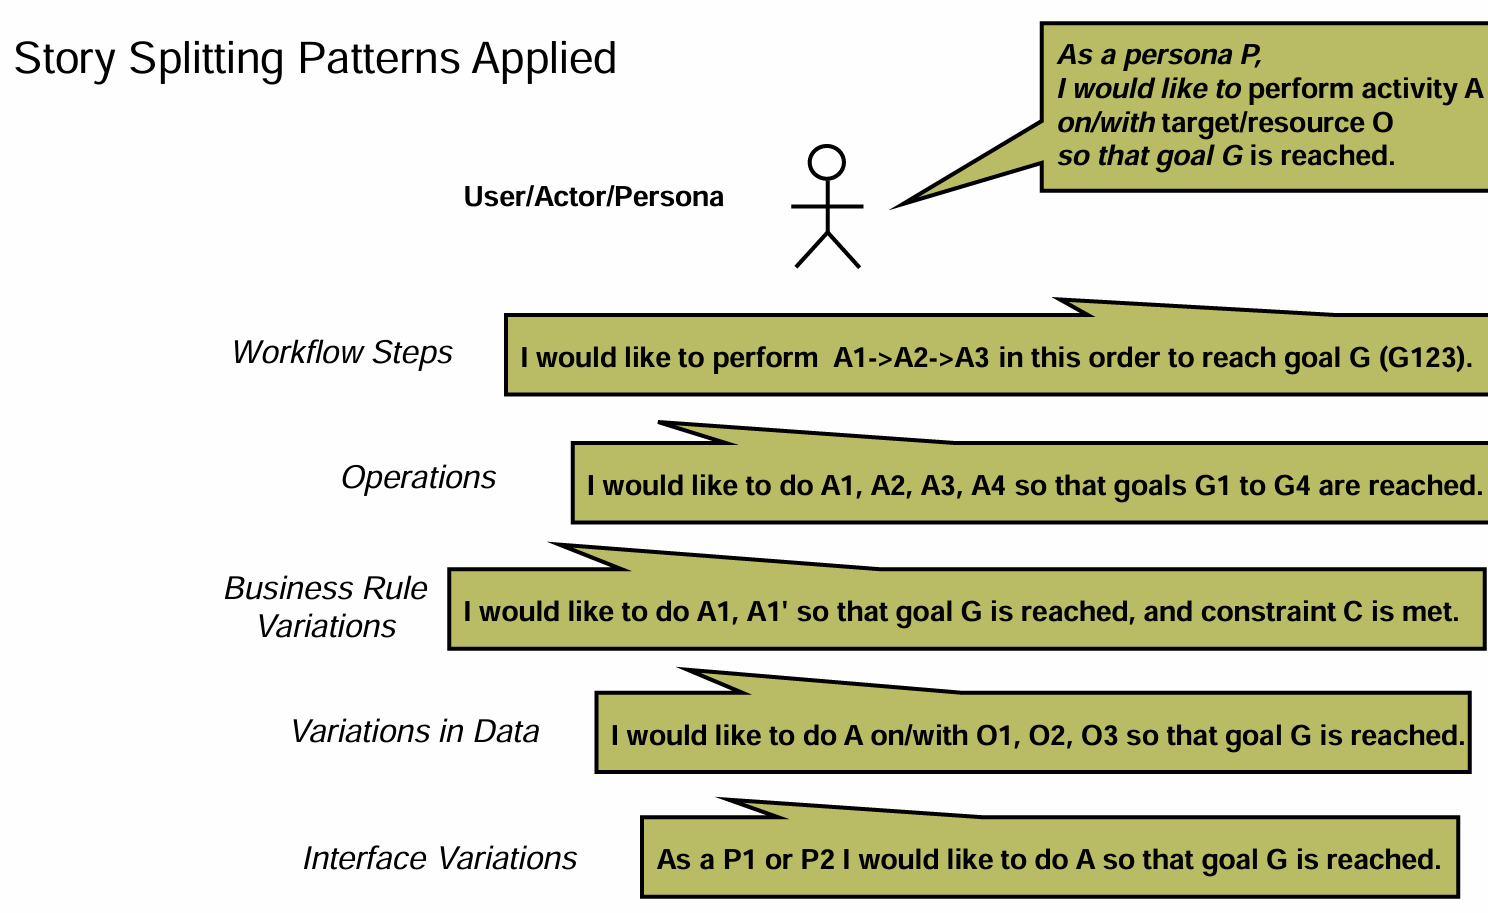
\includegraphics{Images/appliedstorysplitting.png}
    \caption{Story Splitting Example}
    \label{fig:storyplitex}
\end{figure}

\begin{table}
    \centering
    \begin{tabular}{|c|c|c|c|} \hline 
         Splitting Pattern&  Pres Layer
Responsibility &  Business Logic& Data Access
Persistence Layer\\ \hline 
         Workflow Steps&  &  & \\ \hline 
         Operations&  &  & \\ \hline 
         Business Rule
&  &  & \\ \hline 
          Data Variations&  &  & \\ \hline 
 Interface Variations& & &\\ \hline
    \end{tabular}
    \caption{Story Splitting Example Table}
    \label{tab:storysplitex}
\end{table}

\section{AB CHAPTER??? 5-6-7??}
\end{document}
